\section{Framework}
\label{sec:framework}

This section develops the central result: a per-cycle coverage certificate for
the closed loop whose terms map one-to-one onto the three constituent modules,
together with the constraint that renders it enforceable inside a real-time
optimizer. We first fix the loop and the event we certify, introduce the
dimensionless coordinate in which the optimizer's decisions move the modules'
operating regime, state the per-module conditional coverage these regimes
inherit, resolve the objection that feedback voids conformal validity, compose
the modules into a single certificate, and convert the certificate into an
optimizer constraint.

\subsection{The loop and the certified event}
\label{sec:loop}

\begin{figure}[t]
\centering
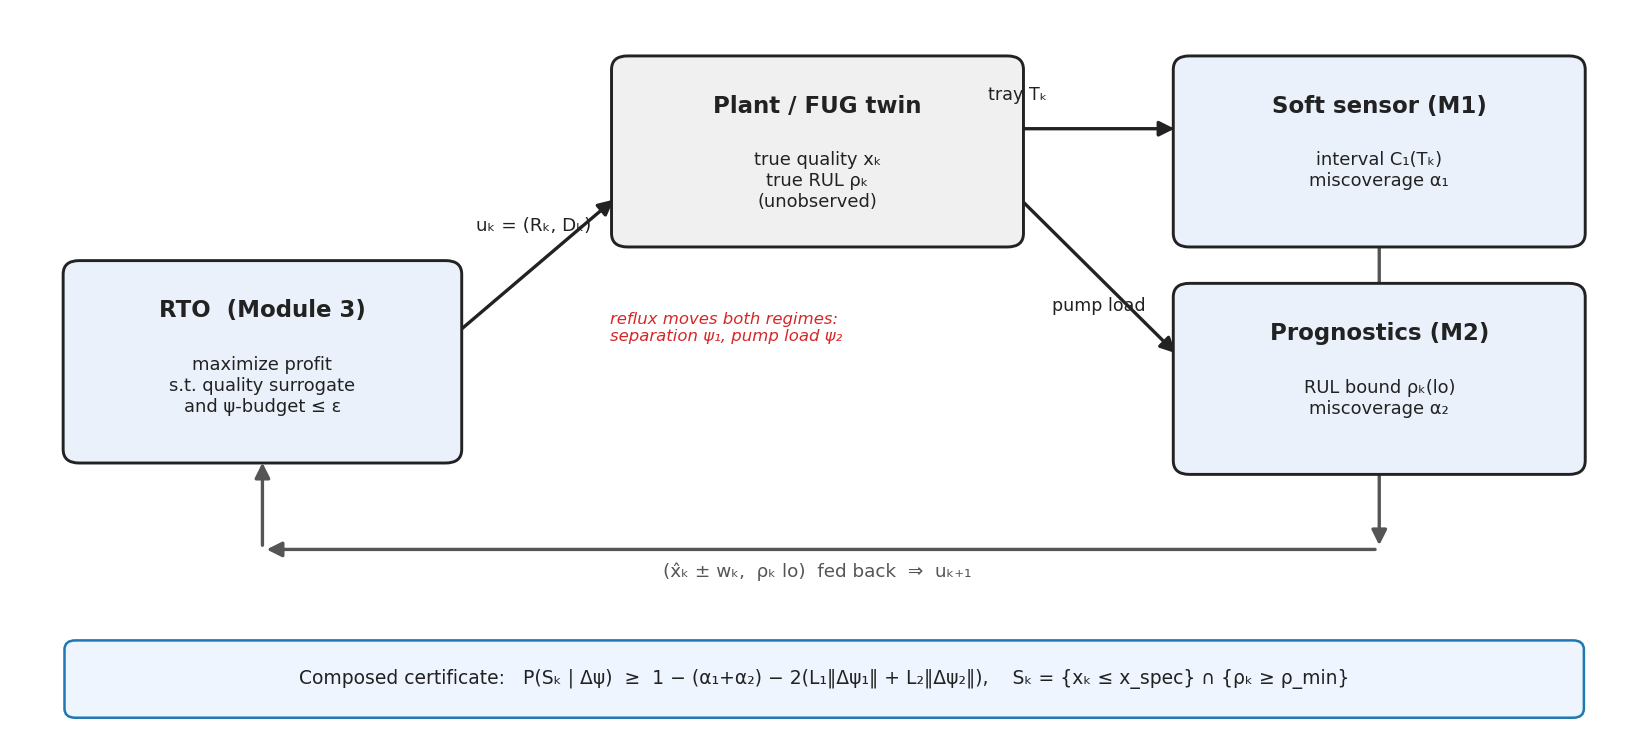
\includegraphics[width=\textwidth]{figures/loop_schematic.png}
\caption{The integrated closed loop. The optimizer (Module~3) sets the decision
$u_k$; the plant returns a tray temperature to the soft sensor (Module~1) and a pump
load to the prognostic module (Module~2), whose interval and remaining-life bound feed
back to the optimizer. The reflux lever moves both modules' operating regimes at once
($\psi_1$ separation, $\psi_2$ pump load), and the composed certificate bounds the
coverage of the joint safety event $S_k$ in terms of the two regime departures.}
\label{fig:loop}
\end{figure}

At control cycle $k$ the real-time optimizer (RTO) sets the decision
$u_k = (R_k, D_k)$, the reflux ratio and distillate rate of a binary-key
distillation column. The plant returns tray temperatures $T_k$ and a true but
\emph{unmeasured} product quality $x_k$, the light-key (C4) mole fraction in the
bottoms. The reflux pump carries a true but \emph{unobserved} remaining useful
life $\rho_k$.

Three modules act on this loop (Figure~\ref{fig:loop}). The soft sensor (Module~1,~\citet{busico_m1})
issues a conformal interval $\hat C_1(T_k) = [\hat x_k - w_k,\, \hat x_k + w_k]$
for the quality with nominal miscoverage $\alpha_1$, so that marginally
$\mathbb{P}(x_k \in \hat C_1(T_k)) \ge 1-\alpha_1$. The prognostic module
(Module~2,~\citet{busico_m2}) issues a one-sided lower bound $\rho_k^{\mathrm{lo}}$
with nominal miscoverage $\alpha_2$, so that
$\mathbb{P}(\rho_k \ge \rho_k^{\mathrm{lo}}) \ge 1-\alpha_2$. The optimizer
(Module~3,~\citet{busico_m3}), a modifier-adaptation
RTO~\citep{marchetti2009,chachuat2009}, computes the next decision while enforcing
two \emph{surrogate} constraints stated on the estimates:
\begin{align}
\hat x_k + w_k &\le x^{\mathrm{spec}}, \label{eq:quality-surrogate}\\
\rho_k^{\mathrm{lo}} &\ge \rho_{\min}, \label{eq:health-surrogate}
\end{align}
where $x^{\mathrm{spec}}$ is the product specification and $\rho_{\min}$ the
remaining life required to reach the next maintenance window. Equation
\eqref{eq:quality-surrogate} backs the spec off by the interval half-width;
\eqref{eq:health-surrogate} is a health floor.

The quantity that actually matters for safe operation is neither estimate but the
joint event on the \emph{truths}: the product is in specification and the pump
survives to maintenance. We call this the system-safety event,
\begin{equation}
S_k \;=\; \{\, x_k \le x^{\mathrm{spec}} \,\} \;\cap\; \{\, \rho_k \ge \rho_{\min} \,\}.
\label{eq:safety-event}
\end{equation}
The surrogate constraints \eqref{eq:quality-surrogate}--\eqref{eq:health-surrogate}
act on estimates; safety \eqref{eq:safety-event} is about truths. The bridge from
one to the other is coverage, and the contribution of this paper is to make that
bridge a single, computable, enforceable guarantee.

\subsection{The similitude coordinate and why the optimizer controls it}
\label{sec:psi}

The modules' calibration is regime-dependent: a conformal interval calibrated at
one operating point need not retain its coverage at another. We track the
operating point in a dimensionless coordinate $\psi$ spanned by three standard
distillation quantities, each verified against Perry's Handbook~\citep{perrys}:
the relative volatility $\alpha(T)$ (Eq.~13-33), the Gilliland reflux coordinate
$\Psi_G = (R - R_{\min})/(R+1)$ (Eq.~13-30, Fig.~13-29), and the stripping factor
$S = KV/L$ (Eq.~13-44). Let $\psi_1\!\star$ and $\psi_2\!\star$ be the anchor
regimes at which Module~1 and Module~2 were calibrated, and define the residual
similitude departures
\begin{equation}
\Delta\psi_{1,k} = \psi_1(u_k) - \psi_1\!\star, \qquad
\Delta\psi_{2,k} = \psi_2(u_k) - \psi_2\!\star,
\label{eq:departure}
\end{equation}
the part of the regime shift not already absorbed by each module's internal
normalizer.

The key structural fact is that \emph{both} departures are functions of the
optimizer's decision. Raising the reflux ratio $R = L/D$ raises the reflux flow
$L$, which raises the reflux-pump duty; the pump-affinity laws (Perry's
Table~10-13: $Q \propto N$, $H \propto N^2$, $\mathrm{BHP} \propto N^3$) map flow
to mechanical load, and Module~2's degradation model maps load to wear. Their
composition makes $\psi_2(u_k)$ a function of $u_k$. The separation departure
$\psi_1(u_k)$ is a function of $u_k$ by construction. Thus the same lever that
the optimizer pulls for economic gain --- reflux --- simultaneously moves both
modules away from the regimes where their guarantees were calibrated. This endogeneity is the source of the difficulty in the next subsection and the
source of the controllability in the $\psi$-budget constraint developed below.

\subsection{Per-module conditional coverage}
\label{sec:permodule}

Within a single cycle the operating regime is held fixed while the modules
predict. The similarity-calibrated conformal certificate of~\citet{busico_m3},
applied conditionally on the cycle's own realized departure, gives
\begin{align}
\mathbb{P}\!\left(x_k \in \hat C_1(T_k) \,\middle|\, \Delta\psi_{1,k}\right)
  &\ge 1-\alpha_1 - 2L_1\|\Delta\psi_{1,k}\|, \label{eq:m1-cond}\\
\mathbb{P}\!\left(\rho_k \ge \rho_k^{\mathrm{lo}} \,\middle|\, \Delta\psi_{2,k}\right)
  &\ge 1-\alpha_2 - 2L_2\|\Delta\psi_{2,k}\|, \label{eq:m2-cond}
\end{align}
where $L_j$ is the Lipschitz constant of the score-quantile map in $\psi$-space,
estimated a~priori from a calibration sweep. The penalty $2L_j\|\Delta\psi_{j,k}\|$
is a physically computable instance of the non-exchangeability coverage gap of
\citet{barber2023}: their abstract distributional distance between calibration and
test is replaced here by the similitude departure, an engineering quantity known
in closed form from the operating point. We write
$E_{1,k} = \{x_k \in \hat C_1(T_k)\}$ and
$E_{2,k} = \{\rho_k \ge \rho_k^{\mathrm{lo}}\}$ for the two coverage events.

\subsection{Why feedback does not break the certificate}
\label{sec:causal}

Because $u_{k+1}$ is computed from $(\hat x_k, \rho_k^{\mathrm{lo}})$, the departure
sequence $\{\Delta\psi_{j,k}\}$ is endogenous, dependent, and controlled, and the
cycle-$k$ test point is not exchangeable with the offline calibration set. This is
the standard reason conformal guarantees are doubted under feedback. The objection
is resolved in two parts.

First, \emph{conditioning}. The bounds \eqref{eq:m1-cond}--\eqref{eq:m2-cond} are
conditional on $\Delta\psi_{j,k}$ and are agnostic to the mechanism that produced
the regime. Endogeneity makes $\Delta\psi_{j,k}$ random; it does not invalidate a
statement already conditioned on it.

Second, \emph{causal timing}. We make explicit the timing assumption that the
closed loop must satisfy.
\begin{assumption}[Causal two-step timing]
\label{ass:causal}
The decision $u_k$ is $\sigma(\mathcal{F}_{k-1})$-measurable --- a function of
information available strictly before cycle $k$ --- and the cycle-$k$ measurement
noise $\varepsilon_k$ satisfies $\varepsilon_k \perp \mathcal{F}_{k-1}$.
\end{assumption}
Under Assumption~\ref{ass:causal}, $u_k$ and $\varepsilon_k$ are conditionally
independent given $\Delta\psi_k$ (itself a function of $u_k$), so conditioning on
the regime leaves $\varepsilon_k$ at its nominal regime-conditional distribution:
\begin{equation}
u_k \perp \varepsilon_k \,\big|\, \Delta\psi_k \;\;\Longrightarrow\;\; \Delta_{\mathrm{sel},k} = 0,
\label{eq:no-selection}
\end{equation}
where $\Delta_{\mathrm{sel},k}$ is a selection penalty that is nonzero only in the
alternative configuration in which the optimizer co-selects $u_k$ on a quantity
computed from the \emph{same} sample used for the coverage check. This delineates
exactly when the conformal-selection effect of~\citet{busico_m3} is active: under
realistic causal plant timing it vanishes; the framework still names and bounds
it. Assumption~\ref{ass:causal} is not a hope about the implementation --- it is a
property of the synchronous control loop used here, which reads $u_k$ from the
solution computed at the close of cycle $k-1$, applies it, and only then realizes
the cycle-$k$ measurement, so that the decision is constructed before the noise it
is conditioned against.

\subsection{The composed certificate}
\label{sec:theorem}

\begin{theorem}[Composed coverage certificate]
\label{thm:composed}
Suppose the optimizer enforces the surrogate constraints
\eqref{eq:quality-surrogate}--\eqref{eq:health-surrogate}, the per-module
conditional bounds \eqref{eq:m1-cond}--\eqref{eq:m2-cond} hold, and
Assumption~\ref{ass:causal} holds. Then the system-safety event
\eqref{eq:safety-event} satisfies, conditionally on the cycle's realized
departures,
\begin{equation}
\mathbb{P}\!\left(S_k \,\middle|\, \Delta\psi_{1,k}, \Delta\psi_{2,k}\right)
\;\ge\; 1 - (\alpha_1 + \alpha_2)
       - 2\!\left(L_1\|\Delta\psi_{1,k}\| + L_2\|\Delta\psi_{2,k}\|\right),
\label{eq:certificate-cond}
\end{equation}
and, marginalizing over the endogenous regime,
\begin{equation}
\mathbb{P}(S_k) \;\ge\; 1 - (\alpha_1 + \alpha_2)
       - 2\!\left(L_1\,\mathbb{E}\|\Delta\psi_{1,k}\| + L_2\,\mathbb{E}\|\Delta\psi_{2,k}\|\right).
\label{eq:certificate-marg}
\end{equation}
\end{theorem}

\begin{proof}
On the enforced surrogate, each coverage event implies its safety half. If
$E_{1,k}$ holds then $x_k \le \hat x_k + w_k \le x^{\mathrm{spec}}$ by
\eqref{eq:quality-surrogate}; if $E_{2,k}$ holds then
$\rho_k \ge \rho_k^{\mathrm{lo}} \ge \rho_{\min}$ by \eqref{eq:health-surrogate}.
Hence $E_{1,k}\cap E_{2,k} \subseteq S_k$, and so
$\mathbb{P}(S_k \mid \cdot) \ge \mathbb{P}(E_{1,k}\cap E_{2,k}\mid\cdot)$.
By the union bound applied to the complementary miscoverage events,
$\mathbb{P}(E_{1,k}\cap E_{2,k}\mid\cdot) \ge 1 - \mathbb{P}(E_{1,k}^c\mid\cdot)
- \mathbb{P}(E_{2,k}^c\mid\cdot)$. Substituting
\eqref{eq:m1-cond}--\eqref{eq:m2-cond}, and using
$\Delta_{\mathrm{sel},k}=0$ from \eqref{eq:no-selection} so the conditional
miscoverages are exactly those of the offline calibration, gives
\eqref{eq:certificate-cond}. Taking expectations over $\Delta\psi_{1,k},
\Delta\psi_{2,k}$ and applying Jensen's inequality to the (linear) departure terms
yields \eqref{eq:certificate-marg}.
\end{proof}

Equation \eqref{eq:certificate-cond} is the unification. Its terms map one-to-one
onto the three modules (Table~\ref{tab:terms}): the base coverage of $\hat C_1$ is
Module~1; the one-sided RUL bound and its miscoverage $\alpha_2$ are Module~2; the
similitude-departure penalty $2L_j\|\Delta\psi_{j,k}\|$ is the per-module,
per-cycle instance of the Module~3 certificate; and the (here vanishing) selection
penalty $\Delta_{\mathrm{sel},k}$ is the Module~3 conformal-selection effect, active
only when the optimizer co-selects on the test residual. No single module states
this inequality; the composition is the contribution.

\begin{table}[t]
\centering
\caption{Each term of the composed certificate \eqref{eq:certificate-cond}
originates in a distinct module.}
\label{tab:terms}
\begin{tabular}{ll}
\toprule
Term & Origin \\
\midrule
$\alpha_1$ (base coverage of $\hat C_1$) & Module~1 --- conformal soft sensor \\
$\alpha_2$ and the one-sided RUL bound & Module~2 --- calibrated prognostics \\
$2L_j\|\Delta\psi_{j,k}\|$ (similitude departure) & Module~3 --- SCC certificate, per cycle \\
$\Delta_{\mathrm{sel},k}$ (selection penalty) & Module~3 --- selection effect, $=0$ here \\
\bottomrule
\end{tabular}
\end{table}

\subsection{The $\psi$-budget constraint}
\label{sec:budget}

Because each departure $\Delta\psi_{j,k} = \psi_j(u_k) - \psi_j\!\star$ is a known
function of the decision $u_k$, the coverage penalty in
\eqref{eq:certificate-cond} is itself controllable. Imposing the single convex
constraint
\begin{equation}
2\!\left(L_1\|\psi_1(u) - \psi_1\!\star\| + L_2\|\psi_2(u) - \psi_2\!\star\|\right) \;\le\; \varepsilon
\label{eq:psi-budget}
\end{equation}
inside the modifier-adaptation NLP yields the following.

\begin{corollary}[Certified floor]
\label{cor:floor}
Under the hypotheses of Theorem~\ref{thm:composed}, if the optimizer additionally
enforces \eqref{eq:psi-budget}, then for every cycle
\begin{equation}
\mathbb{P}(S_k) \;\ge\; 1 - (\alpha_1 + \alpha_2) - \varepsilon.
\label{eq:floor}
\end{equation}
\end{corollary}

\begin{proof}
Constraint \eqref{eq:psi-budget} bounds the departure term in
\eqref{eq:certificate-cond} by $\varepsilon$ for every realized $u_k$, hence for
every realized $(\Delta\psi_{1,k},\Delta\psi_{2,k})$; the bound
\eqref{eq:floor} then holds conditionally and therefore marginally.
\end{proof}

Corollary~\ref{cor:floor} converts the certificate into an operating rule: the
optimizer maximizes economic profit \emph{subject to remaining inside the
similitude-departure budget that certifies its own coverage} --- formally, it may
not optimize so aggressively that it invalidates its own soft sensor and its own
RUL guarantee. The radius $\varepsilon$ is the chosen coverage budget, traded
directly against economics. Theorem~\ref{thm:composed} and
Corollary~\ref{cor:floor} share one implementation: the flagship per-cycle
guarantee and the operational floor are the same constraint
\eqref{eq:psi-budget} added to the NLP.
